\begin{frame}{The basics (1): What is git?}
  \begin{columns}[onlytextwidth]
    \begin{column}{0.6\textwidth}
      \begin{itemize}
        \item git -- ``the stupid content tracker''
        \begin{itemize}
          \item open-source version control system
          \item fast, scalable, distributable
        \end{itemize}
        \item originally developed in 2005 for maintaining the linux kernel source code
      \end{itemize}
    \end{column}
    \begin{column}[t]{0.4\textwidth}
      
\includegraphics[width=0.95\textwidth]{imgs/git_logo}
    \end{column}
  \end{columns}
\end{frame}

\begin{frame}{The basics (2): Working directory, index \& repository}
  \begin{columns}[onlytextwidth]
    \begin{column}{0.6\textwidth}
      \begin{itemize}
        \item git maintains multiple versions of a project
        \item each repository has
        \begin{itemize}
          \item a working directory (where files are editable)
          \item a staging area (also called index)
          \item a git directory (contains all the history of the repository)
        \end{itemize}
        \item basic commands
        \begin{itemize}
          \item git add, git commit, git checkout
        \end{itemize}
      \end{itemize}
    \end{column}
    \begin{column}[c]{0.4\textwidth}
      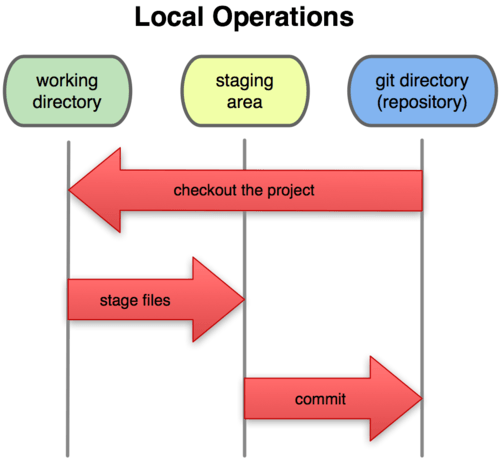
\includegraphics[width=0.95\textwidth]{imgs/git_local}
    \end{column}
  \end{columns}
\end{frame}